\documentclass{article}
\usepackage{geometry}
 \geometry{
 a4paper,
 total={210mm,297mm},
 left=20mm,
 right=20mm,
 top=20mm,
 bottom=20mm,
 }

\usepackage{siunitx} % Provides the \SI{}{} command for typesetting SI units
\usepackage{listings}
\usepackage{graphicx} % Required for the inclusion of images
\usepackage{enumerate}
\usepackage{float}
\usepackage{fancyvrb}
\usepackage[utf8]{inputenc}
\usepackage{listings}
\usepackage{inconsolata}
\usepackage{placeins}
\usepackage{subcaption}
\usepackage[draft]{fixme}
\usepackage{float}
\usepackage{fontawesome}

\usepackage{hyperref}
\hypersetup{
  colorlinks   = true,    % Colours links instead of ugly boxes
  urlcolor     = blue,    % Colour for external hyperlinks
  linkcolor    = blue,    % Colour of internal links
  citecolor    = red      % Colour of citations
}

\newcommand{\codelink}[1]{%
    \hyperref[#1]{\faArrowCircleRight\enskip Matlab Code (Listing~\ref{#1})}%
}

\lstset{
    frame=single,
    basicstyle=\small\ttfamily,
    language=bash
}

\setlength\parindent{0pt} % Removes all indentation from paragraphs

\title{Network Security \\ 389.159 - SS 2018 \\ Lab Exercise 3 \& Lab Exercise 4} % Title

\author{
    TEAM 02 \\
    Corentin \textsc{Bergès} (11741629) (066 506) \\
    Christoph \textsc{Echtinger-Sieghart} (00304130) (066 938)
}

\date{\today} % Date for the report
\begin{document}

\maketitle % Insert the title, author and date
\renewcommand{\arraystretch}{2} %Stretch rows

\listoffixmes

\section{Lab Exercise 3}

\subsection{rep-10 }

\codelink{code:rep-10}

Figure~\ref{figure:rep-10} shows the stem plots for packets, bytes, unique IP sources and
unique IP destinations per hour.

\begin{figure}[H]
    \begin{subfigure}{.5\textwidth}
        \centering
        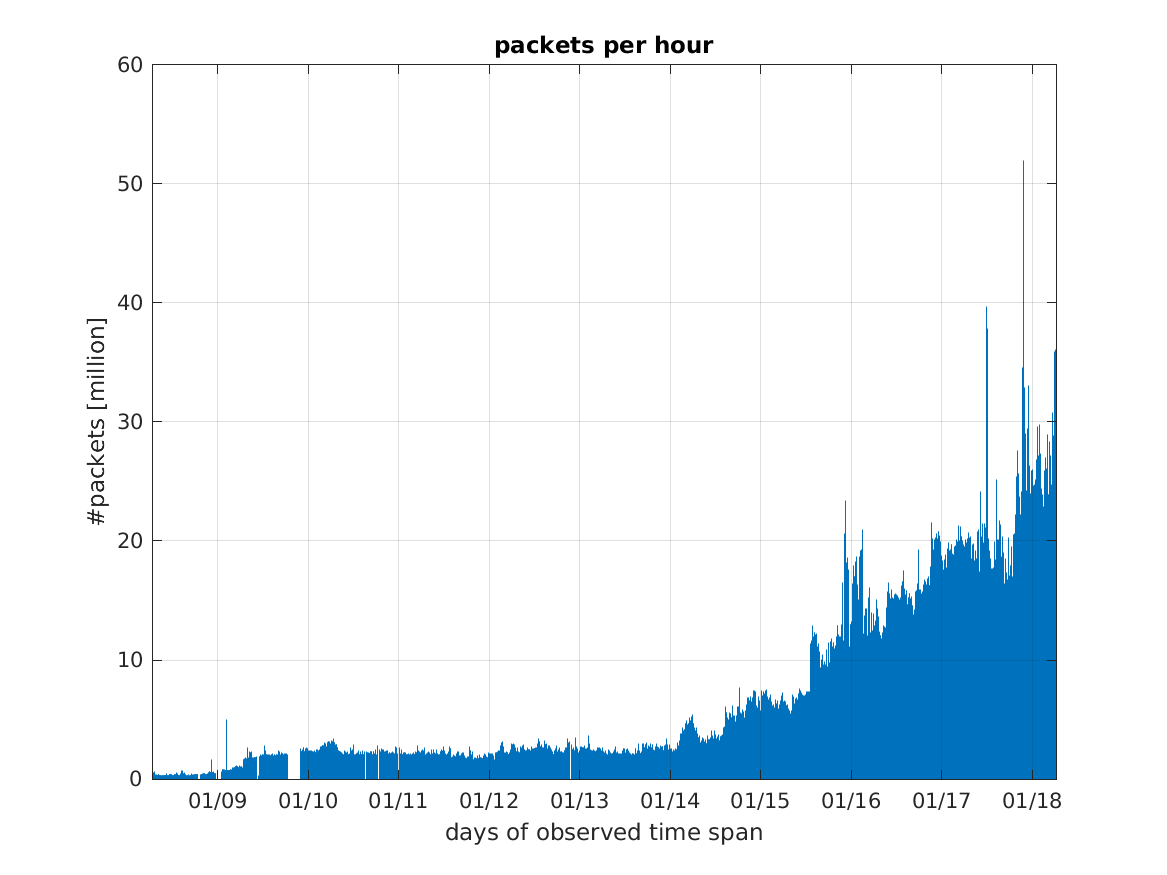
\includegraphics[width=\textwidth]{../exercise-3/plots/rep_10_1}
        \caption{Packets per hour}
    \end{subfigure}
    \begin{subfigure}{.5\textwidth}
        \centering
        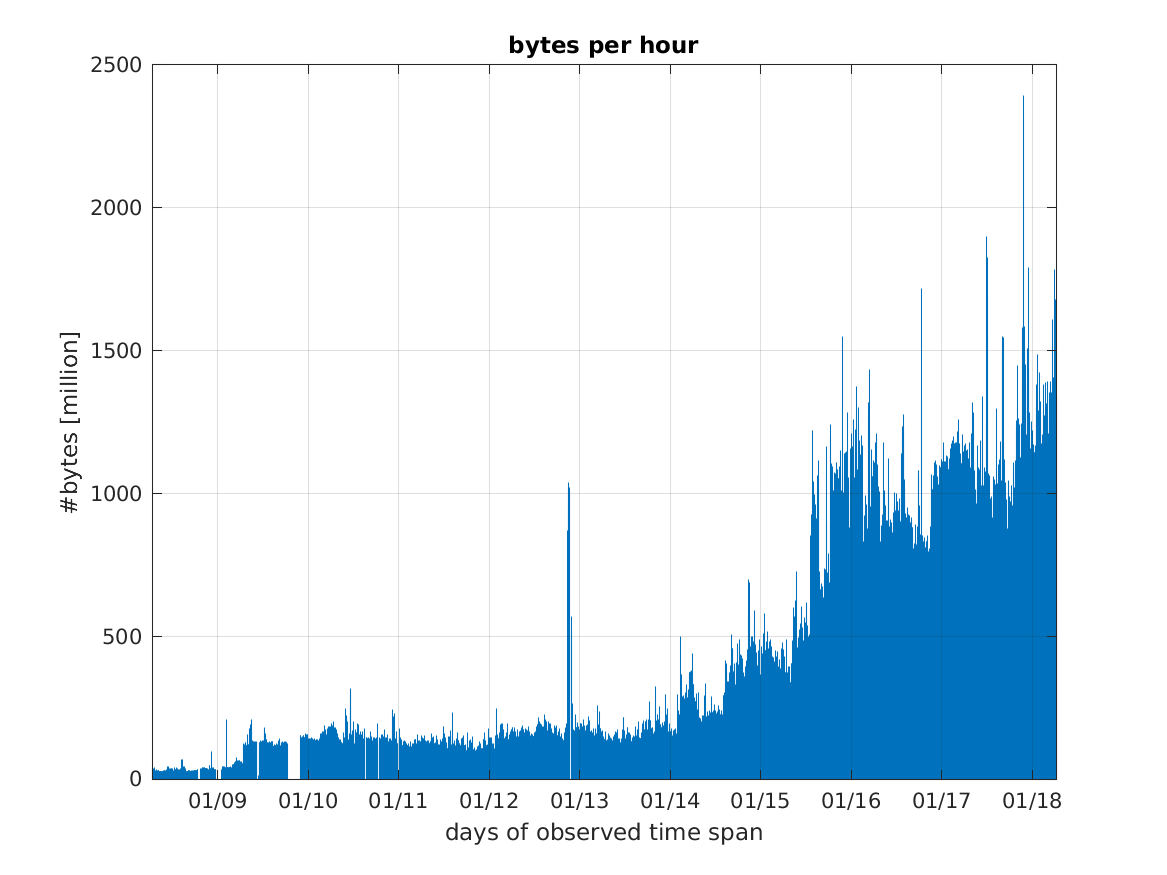
\includegraphics[width=\textwidth]{../exercise-3/plots/rep_10_2}
        \caption{Bytes per hour}
    \end{subfigure}
    \begin{subfigure}{.5\textwidth}
        \centering
        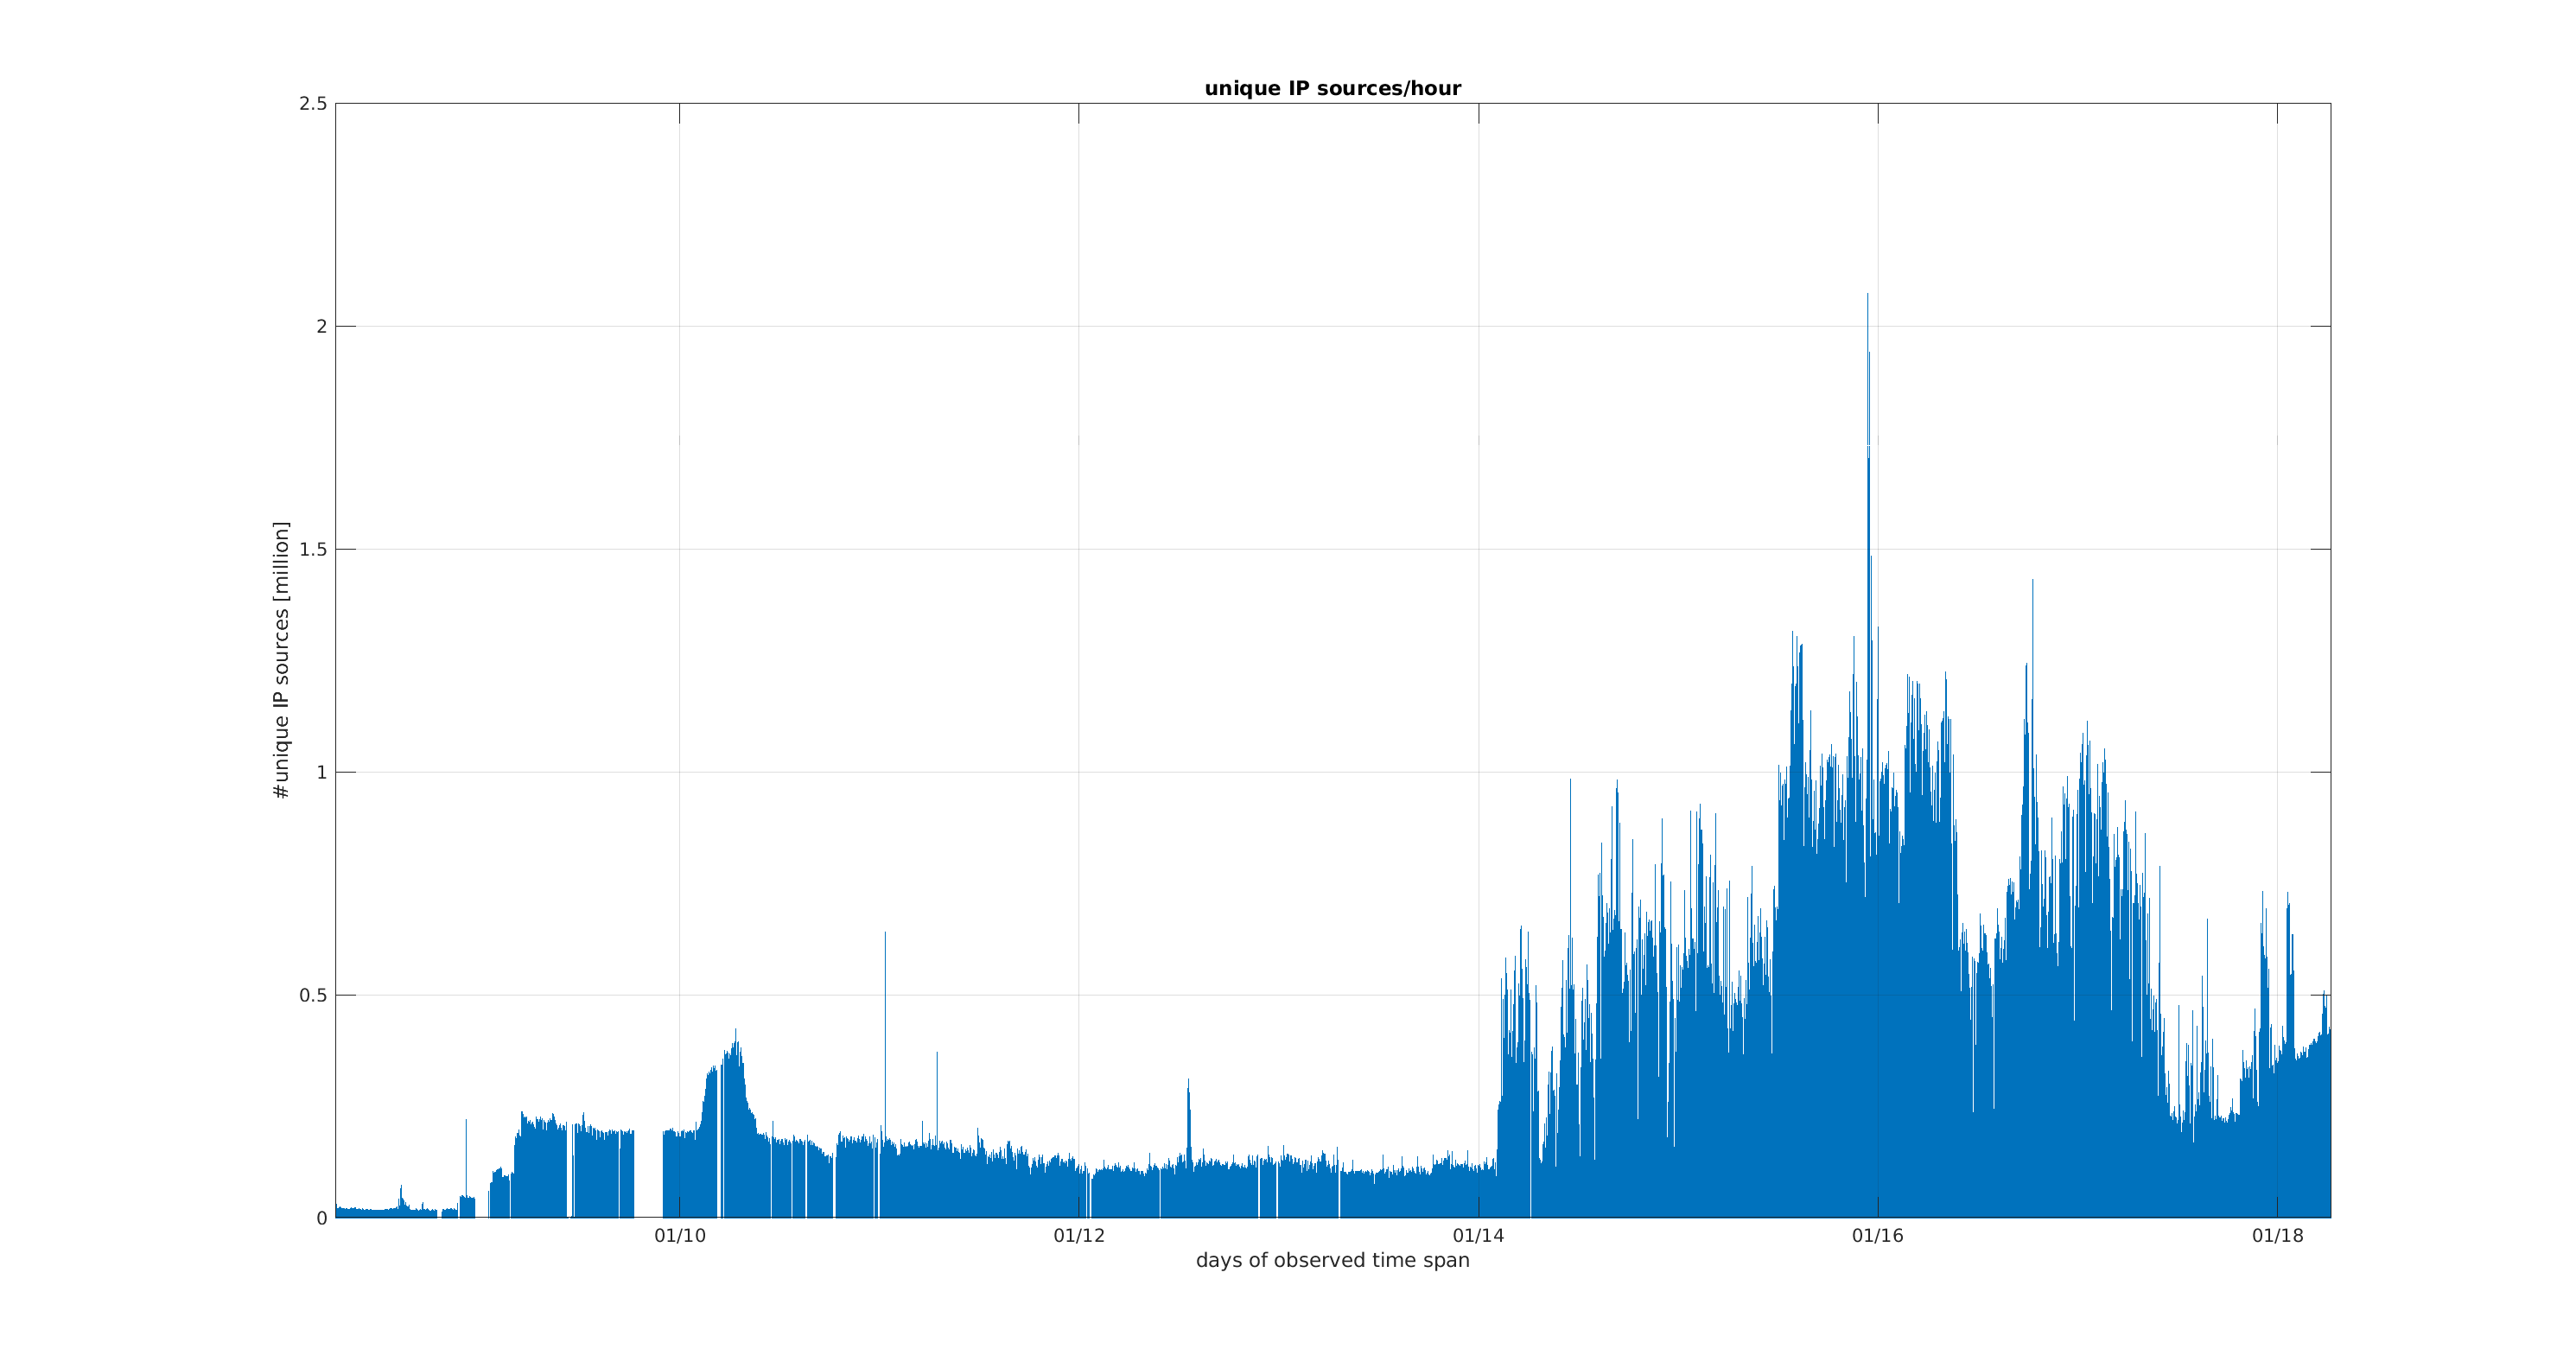
\includegraphics[width=\textwidth]{../exercise-3/plots/rep_10_3}
        \caption{IP sources per hour}
    \end{subfigure}
    \begin{subfigure}{.5\textwidth}
        \centering
        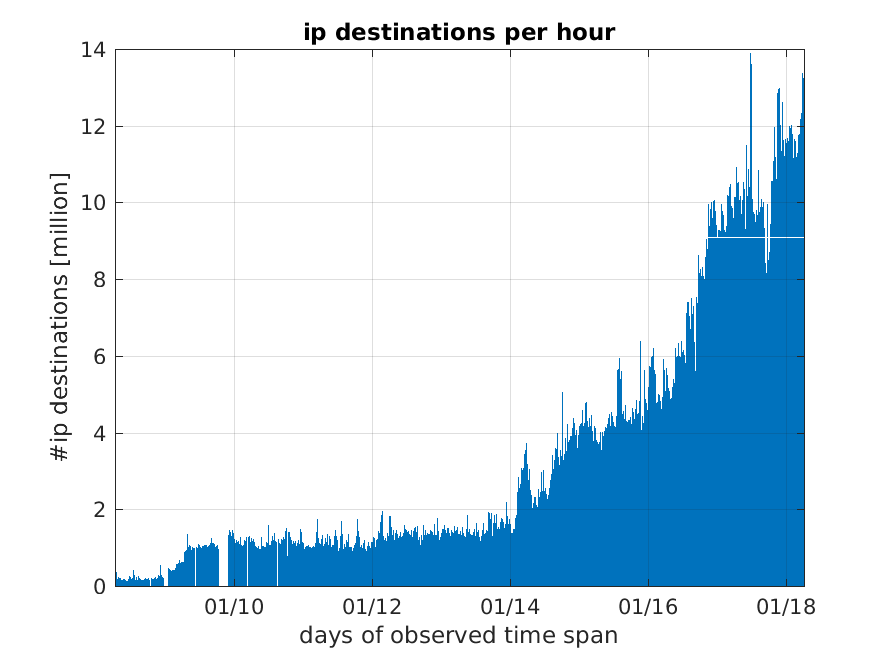
\includegraphics[width=\textwidth]{../exercise-3/plots/rep_10_4}
        \caption{IP destinations per hour}
    \end{subfigure}
    \caption{\label{figure:rep-10}}
\end{figure}

\paragraph{Optional}

Figure~\ref{figure:rep-10-optional} shows all signals from Figure~\ref{figure:rep-10} combined, normalized
and smoothed with a moving average filter.

\begin{figure}[H]
    \centering
    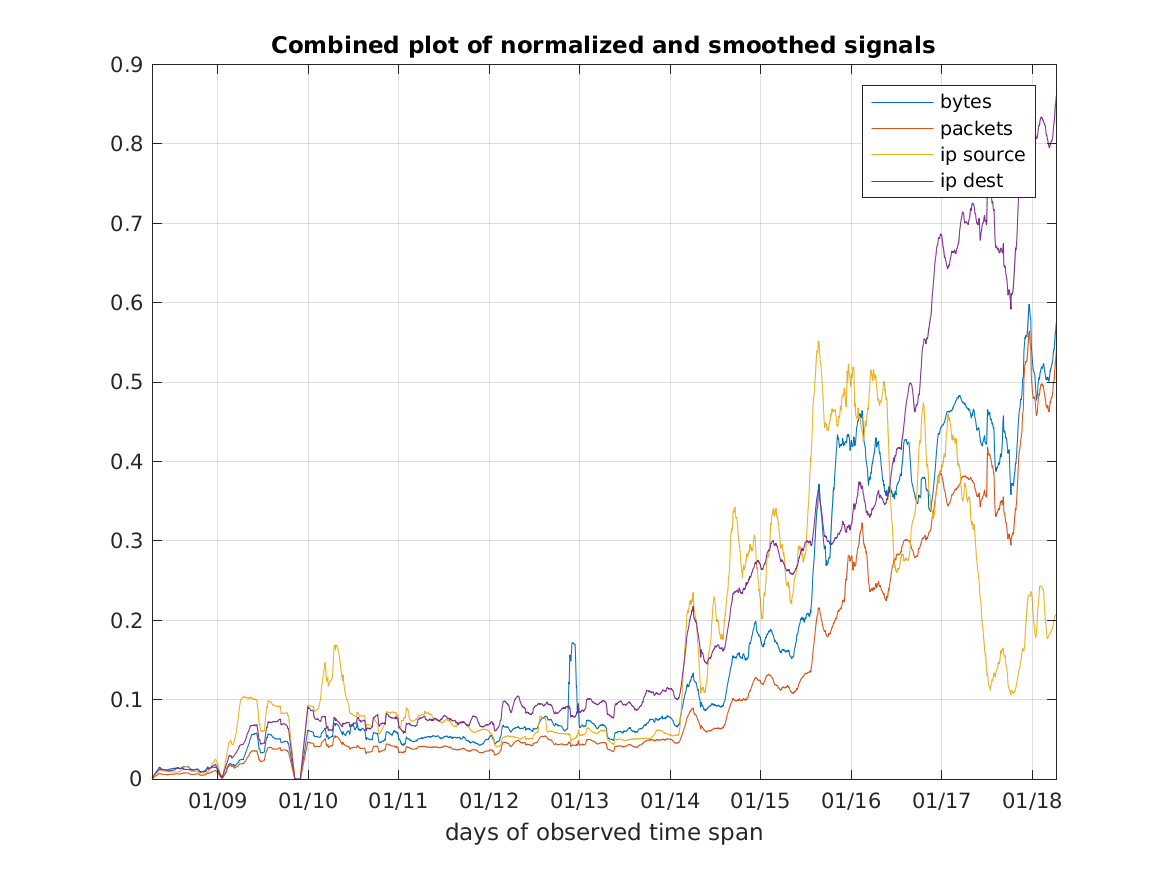
\includegraphics[width=\textwidth]{../exercise-3/plots/rep_10_optional}
    \caption{\label{figure:rep-10-optional} Combined, normalized and smoothed signals}
\end{figure}

\subsection{rep-11}

\codelink{code:rep-11}

The signal that shows the lower correlation to the other signals is \textbf{IP sources}. The minimum
linear correlation coefficient is \textbf{0.588568} between the signals \textbf{IP sources} and
\textbf{IP destinations}. See Table~\ref{table:rep-11} for the raw data.

\begin{table}[h]
    \centering
    \begin{tabular}{l|c|c|c|c}
                & Bytes  & Packets& IP src    & IP dst    \\
        \hline
        Bytes   & 1      & 0.9655 & 0.7203 & 0.9340 \\
        Packets & 0.9655 & 1      & 0.6105 & 0.9732 \\
        IP src     & 0.7203 & 0.6105 & 1      & 0.5886 \\
        IP dst     & 0.9340 & 0.9732 & 0.5886 & 1      \\
    \end{tabular}
    \caption{\label{table:rep-11} Correlation coefficients between signals}
\end{table}

The reason for why the drop in unique IP sources does not cause a proportional drop in the other
signals, could be that many small attackers (botnets), that did not contribute a lot to the other
signals somehow stopped sending traffic.

\subsection{rep-12}

\codelink{code:rep-12}

The number of IP sources is bigger in average than the number of darkspace addresses
receiving packets. There are on average around ten times more IP sources than IP destinations.
This makes sense, because the darkspace is only a small part of the internet address-space, but
the IP sources are taken from the whole address-space.

\subsection{rep-13}
\codelink{code:rep-13}

The main peak in IP sources starts on 14-Dec-2015 and lasts until 16-Dec-2015. See Table~\ref{table:rep-13}
for the detailed data.

\begin{table}[h]
    \centering
    \begin{tabular}{c|r}
        Date & \# IP sources \\
        \hline
        14-Dec-2015 & 2075358.074306 \\
        15-Dec-2015 & 1704892.012500 \\
        16-Dec-2015 & 1942072.404167 \\
    \end{tabular}
    \caption{\label{table:rep-13} Detailed data for peak in IP sources}
\end{table}

\paragraph{Optional}
\codelink{code:rep-13-optional}
The main peak in Bytes starts on 14-Nov-2012 and lasts until 22-Nov-2012. Note that
on 19-Nov-2012 no data was available. See Table~\ref{table:rep-13-optional}
for the detailed data.

\begin{table}[h]
    \centering
    \begin{tabular}{c|r}
        Date & \# Bytes \\
        \hline
        14-Nov-2012& 870858582.136110 \\ 
        15-Nov-2012& 1009586335.331900 \\
        16-Nov-2012& 1038654926.456100 \\
        17-Nov-2012& 1021464983.022200 \\
        18-Nov-2012& 954193481.914190 \\ 
        20-Nov-2012& 1005163238.508500 \\
        21-Nov-2012& 1020526661.658000 \\
        22-Nov-2012& 989613880.615110  \\
    \end{tabular}
    \caption{\label{table:rep-13-optional} Detailed data for peak in Bytes}
\end{table}

\subsection{rep-14}
\codelink{code:rep-14}

Table~\ref{table:rep-14-daily} gives statistics for the data from
\texttt{global\_last10years.csv}. Table~\ref{table:rep-14-hourly} gives
statistics for the data from \texttt{Feb2017\_gen.csv}.

\begin{table}[h]
    \centering
    \begin{tabular}{l|rrrr}
                & Sum & Mean & Median & StdDev \\
                \hline
        \# Packets [millions] &   146373.391 & 41.845 & 17.699 & 40.916 \\
        \# Bytes [millions]   &    2381.003 & 0.681 & 0.263 & 0.735 \\
        \# IP src [millions]     & 123.613 & 0.035 & 0.020 & 0.031 \\
        \# IP dst  [millions]    & 1150.796 & 0.329 & 0.142 & 0.330 \\
    \end{tabular}
    \caption{\label{table:rep-14-daily} Statistics for daily data}
\end{table}

\begin{table}[h]
    \centering
    \begin{tabular}{l|rrrr}
                & Sum & Mean & Median & StdDev \\
                \hline
        \# Packets [millions] &    76871.319 & 114.392 & 113.464 & 7.033 \\
        \# Bytes  [millions]  &    1272.998  &1.894 & 1.890 & 0.097      \\
        \# IP src  [millions]    & 59.651 & 0.089 & 0.091 & 0.018        \\
        \# IP dst   [millions]   & 619.875 & 0.922 & 0.931 & 0.070       \\
    \end{tabular}
    \caption{\label{table:rep-14-hourly} Statistics for hourly data}
\end{table}

\subsection{rep-15}

The values do not coincide. February 2017 seems to be a month that is not really representative for the
data collected over a span of 10 years.

\paragraph{Optional}
\codelink{code:rep-15-optional}

\begin{figure}[h]
    \centering
    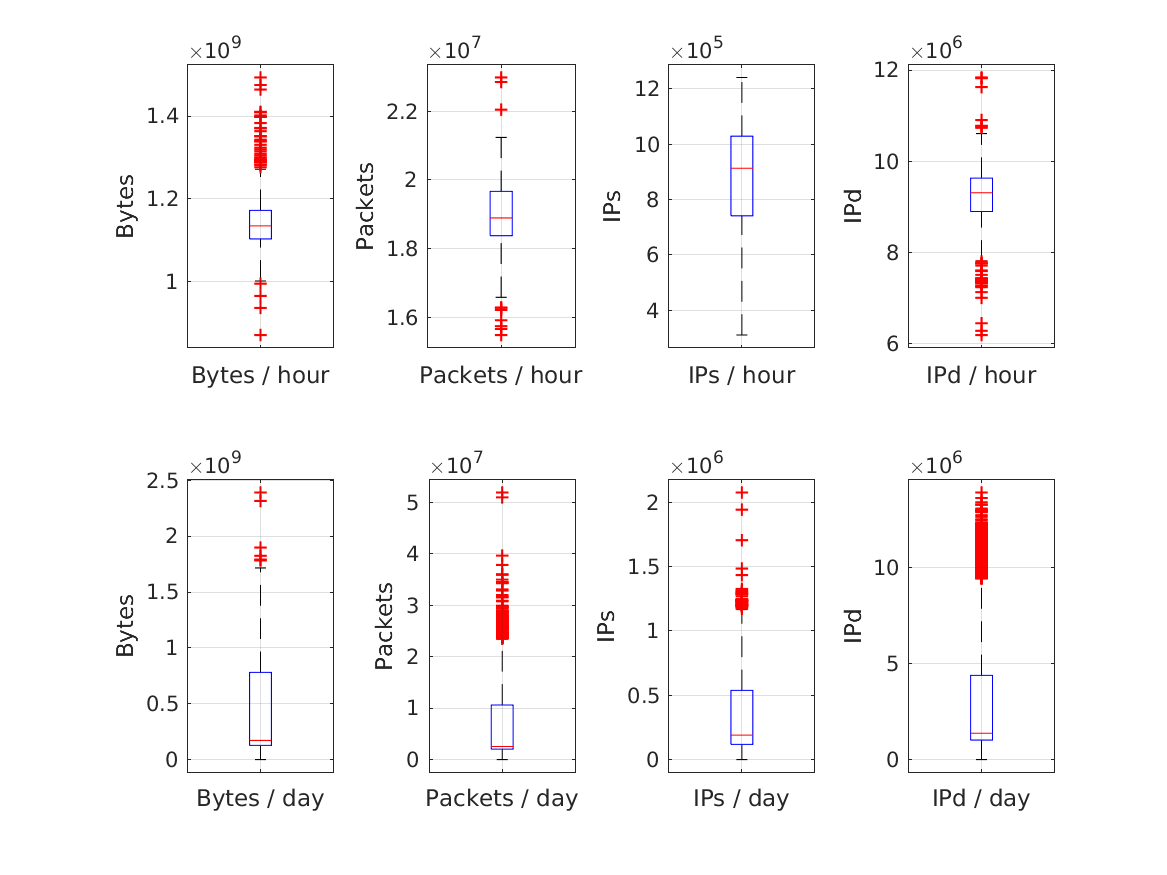
\includegraphics[width=\textwidth]{../exercise-3/plots/rep_15_optional}
    \caption{\label{figure:rep-15-optional} Boxplots for hourly and daily averaged data}
\end{figure}

A difference between the box plots for the hourly and daily data are the positions of
the medians in the plots. The medians in the daily averaged data show a clear tendency to
be in the vicinity of the first quartile, whereas the medians in the hourly averaged data
show no clear tendency.
A second noticeable difference are the outliers. All outliers in the daily averaged data are
above the whiskers, whereas the boxplots for the hourly averaged data show outliers below and
above the whiskers.

\subsection{rep-16}

We used https://www.iana.org/assignments/protocol-numbers/protocol-numbers.xhtml to look up the
protocol numbers.

\paragraph{Protocol 6 (TCP)}
The Transmission Control Protocol is a connection oriented, reliable protocol that is widely used.
A TCP connection is created by performing a three-way handshake (SYN, SYN/ACK, ACK). TCP uses
port numbers to address applications.

\paragraph{Protocol 1 (ICMP)}
The Internet Control Message Protocol is a protocol used to exchange status and error messages
concerning the IP protocol. ICMP is transported via IP. The popular \texttt{ping} and \texttt{traceroute}
programs are applications that make use of ICMP.

\paragraph{Protocol 17 (UDP)}
The User Datagram Protocol is a connectionless, unreliable protocol. UDP does not perform
a three-way handshake, but also uses port numbers to address applications.

\subsection{rep-17}
\codelink{code:rep-17}

Table~\ref{table:rep-17-packets} shows statistical information for Packets/hour grouped by protocol.
Table~\ref{table:rep-17-ips} shows statistical information for IP sources/hour grouped by protocol.
Table~\ref{table:rep-17-ipd} shows statistical information for IP destinations/hour grouped by protocol.

\begin{table}[H]
    \centering
    \begin{tabular}{l|ccc}
               & Mean  & Median & StdDev \\
               \hline
        TCP    & 0.840 & 0.833  & 0.048 \\
        UDP    & 0.114 & 0.113  & 0.032 \\
        ICMP   & 0.043 & 0.054  & 0.026 \\
        Others & 0.004 & 0.004  & 0.001 \\
    \end{tabular}
    \caption{\label{table:rep-17-packets} Statistical information for Packets/hour (percentages)}
\end{table}

\begin{table}[H]
    \centering
    \begin{tabular}{l|ccc}
               & Mean  & Median & StdDev \\
               \hline
        TCP    &   0.592 & 0.519  & 0.143  \\
        UDP    &   0.336 & 0.343  & 0.034  \\
        ICMP   &   0.175 & 0.225  & 0.106  \\
        Others &  -0.103 & -0.103 & 0.044  \\
    \end{tabular}
    \caption{\label{table:rep-17-ips} Statistical information for IP sources/hour (percentages)}
\end{table}

\begin{table}[H]
    \centering
    \begin{tabular}{l|ccc}
               & Mean  & Median & StdDev \\
               \hline
        TCP    &  0.890 & 0.883&  0.039   \\
        UDP    &  0.158 & 0.155&  0.045   \\
        ICMP   &  0.080 & 0.104&  0.048   \\
        Others &  -0.127&  -0.142&  0.042 \\
    \end{tabular}
    \caption{\label{table:rep-17-ipd} Statistical information for IP destinations/hour (percentages)}
\end{table}

\fxerror{boxplot per signal}
%Figure~\ref{figure:rep-17} shows boxplots for the data from \texttt{Feb2017_proto.csv}.

%\begin{figure}[H]
%    \includegraphics[width=\textwidth]{../exercise-3/plots/rep_17}
%    \caption{\label{figure:rep-17} Boxplots for data from \texttt{Feb2017_proto.csv}}
%\end{figure}

\paragraph{Optional}

Figure~\ref{figure:rep-17-optional} shows the various scatter plots.

\begin{figure}[H]
    \begin{subfigure}{.5\textwidth}
        \centering
        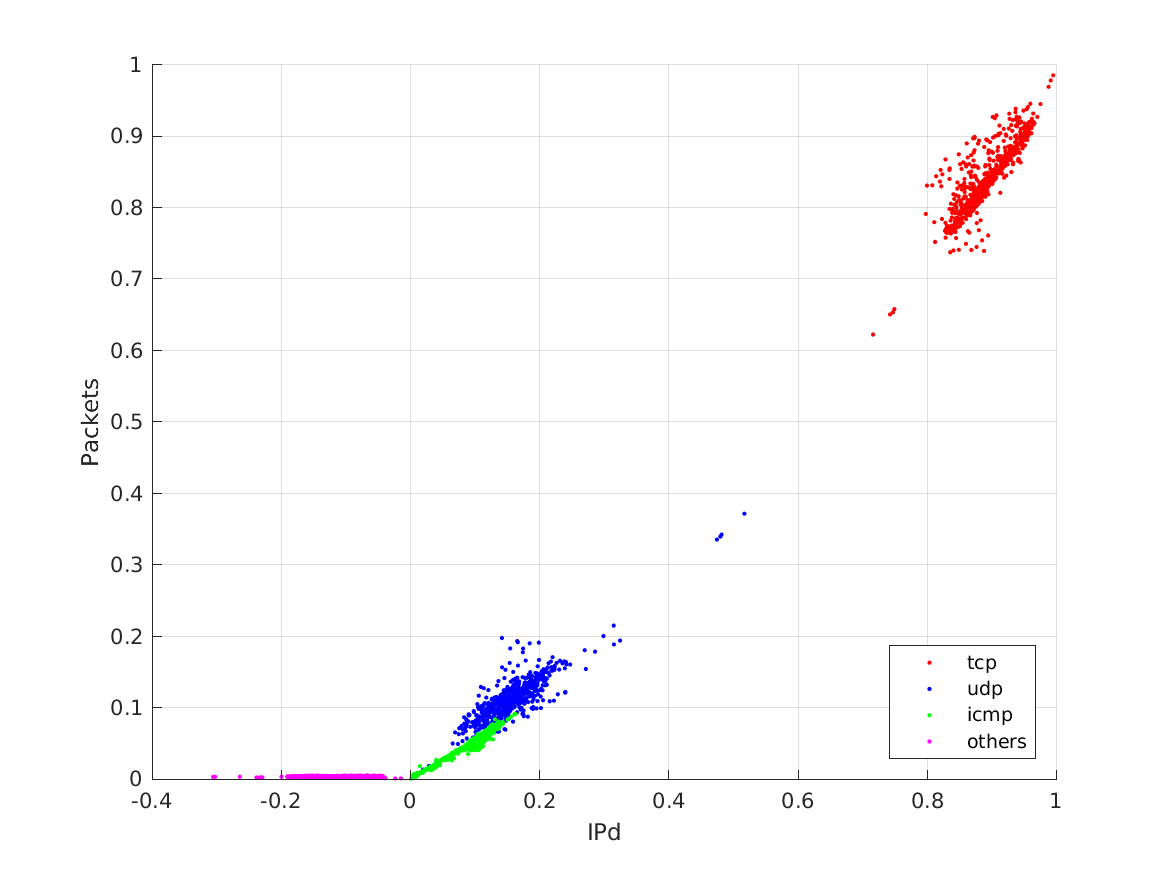
\includegraphics[width=\textwidth]{../exercise-3/plots/rep_17_optional_IPdPackets.png}
        \caption{Packets vs IP destinations}
    \end{subfigure}
    \begin{subfigure}{.5\textwidth}
        \centering
        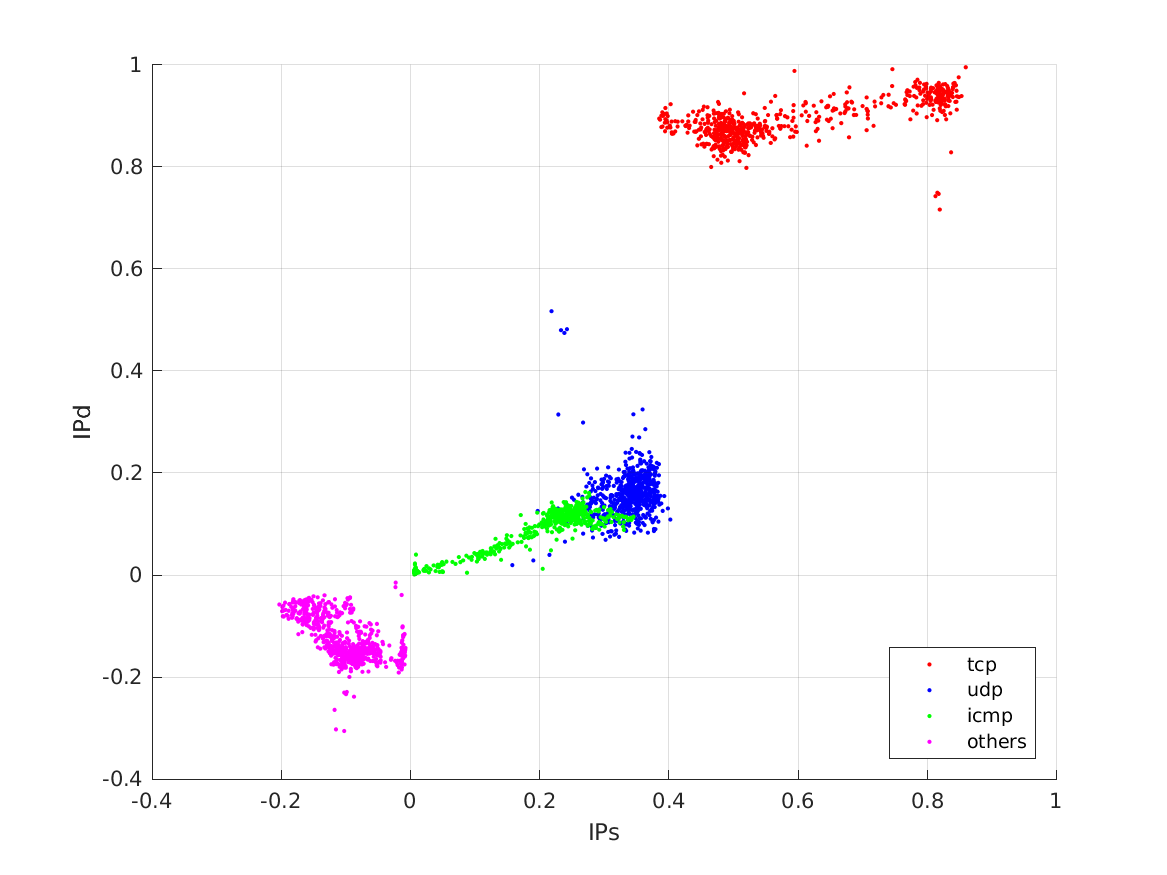
\includegraphics[width=\textwidth]{../exercise-3/plots/rep_17_optional_IPsIPd.png}
        \caption{IP destinations vs IP sources}
    \end{subfigure}
    \begin{subfigure}{.5\textwidth}
        \centering
        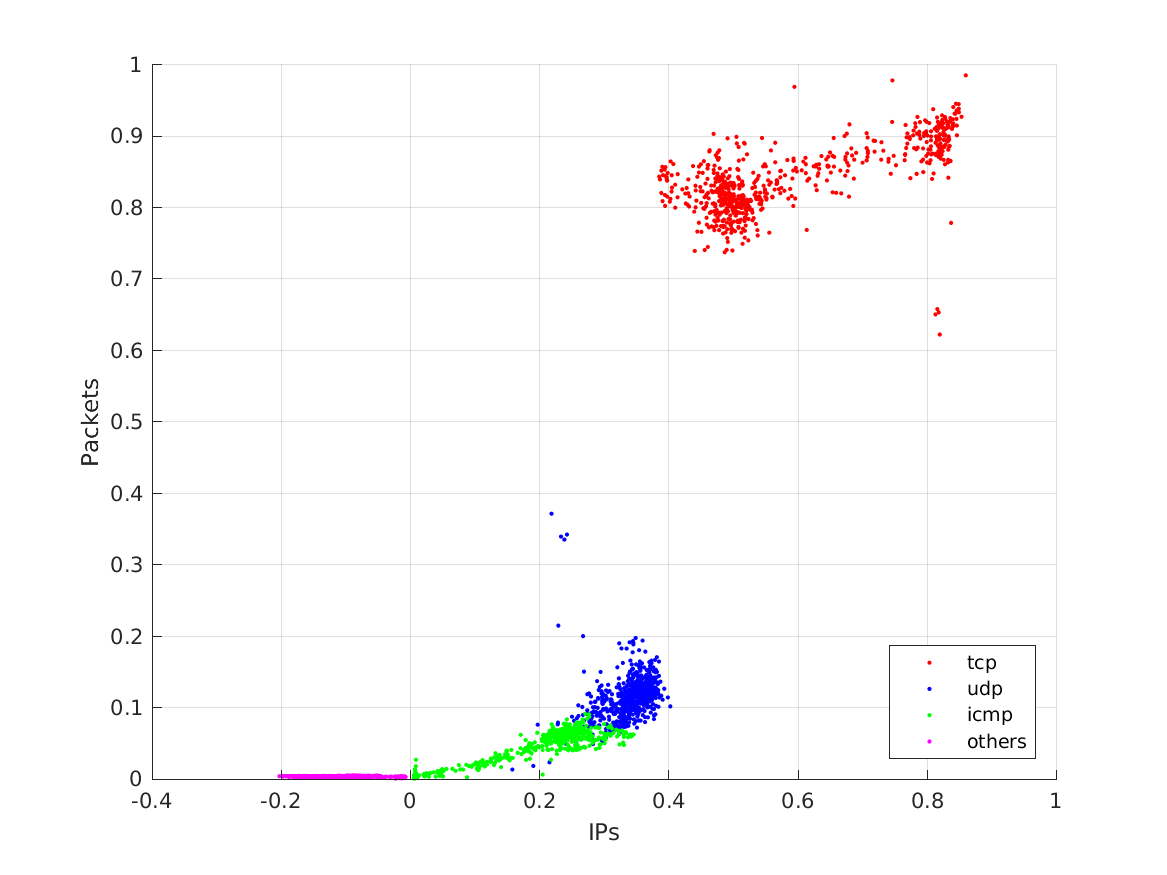
\includegraphics[width=\textwidth]{../exercise-3/plots/rep_17_optional_IPsPackets.png}
        \caption{Packets vs IP sources}
    \end{subfigure}
    \caption{\label{figure:rep-17-optional} Scatter plots}
\end{figure}

\subsection{rep-18}

We obtained negative values for ``Others'' because, in the combined data addresses are collapsed. The same
address might get a TCP, a UDP and an ICMP packet, but will only be counted once.

%optional
\subsection{rep-19}
\codelink{code:rep-19}

%optional
\subsection{rep-20}

\subsection{rep-21}
\subsection{rep-22}
\subsection{rep-23}

\begin{lstlisting}[label=listing:ip-command,caption={Command used to obtain IP address}]
team02@pc01:~$ ip address show dev em1
\end{lstlisting}

\paragraph{Port 113}
\begin{Verbatim}
IP 192.168.83.20.1073 > 192.168.83.33.113: Flags [S], seq 0, win 8192, length 0
IP 192.168.83.33.113 > 192.168.83.20.1073: Flags [R.], seq 0, ack 1, win 0, length 0
\end{Verbatim}

\section{Lab Exercise 4}

\subsection{rep-24}
\subsection{rep-25}
\subsection{rep-26}
\subsection{rep-27}
\subsection{rep-28}
\subsection{rep-29}
\subsection{rep-30}

\FloatBarrier

\appendix
\newpage
\section{Matlab Code}
\lstinputlisting[%
    float,language=Matlab,caption={Matlab code to solve rep-10},label=code:rep-10%
]{../exercise-3/team02_rep10.m}

\lstinputlisting[%
    float,language=Matlab,caption={Matlab code to solve rep-11},label=code:rep-11%
]{../exercise-3/team02_rep11.m}

\lstinputlisting[%
    float,language=Matlab,caption={Matlab code to solve rep-12},label=code:rep-12%
]{../exercise-3/team02_rep12.m}

\lstinputlisting[%
    float,language=Matlab,caption={Matlab code to solve rep-13},label=code:rep-13%
]{../exercise-3/team02_rep13.m}

\lstinputlisting[%
    float,language=Matlab,caption={Matlab code to solve rep-13 optional},label=code:rep-13-optional%
]{../exercise-3/team02_rep13_optional.m}

\lstinputlisting[%
    float,language=Matlab,caption={Matlab code to solve rep-14},label=code:rep-14%
]{../exercise-3/team02_rep14.m}

\lstinputlisting[%
    float,language=Matlab,caption={Matlab code to solve rep-15 optional},label=code:rep-15-optional%
]{../exercise-3/team02_rep15_optional.m}

\lstinputlisting[%
    float,language=Matlab,caption={Matlab code to solve rep-17},label=code:rep-17%
]{../exercise-3/team02_rep17.m}

\lstinputlisting[%
    float,language=Matlab,caption={Matlab code to solve rep-19},label=code:rep-19%
]{../exercise-3/team02_rep19.m}

\end{document}
